\chapter{Background}
\label{chap:Two}
\section{Concepts overview} 
\label{sec:ConceptsOverview}
\subsection{Deep Learning}
\label{sec:DP}
Deep Learning is one of the most emerging techniques in the modern era, as illustrated in figure \ref{figure:DL}.
\begin{figure}[H]
\centering
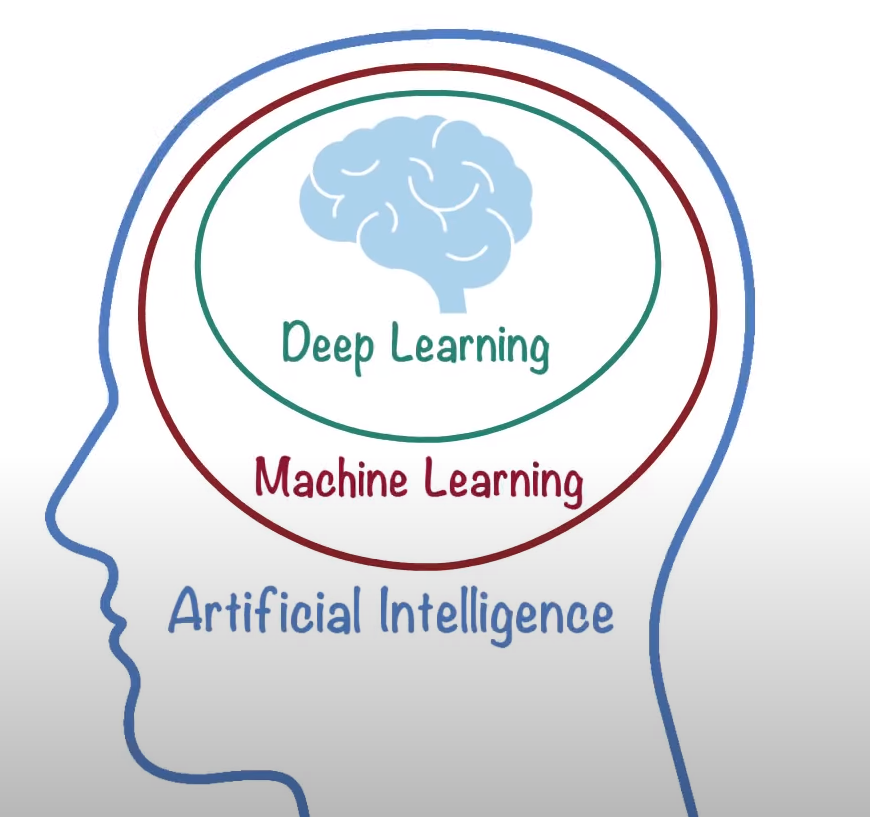
\includegraphics[width=6.5cm]{Figures/DL.PNG}
\caption{Deep Learning as a Subset}
\label{figure:DL}
\end{figure}

  \cite{citeKey8} discusses the development of one of the widely used optimzers in machine learning Adam. Adam is one of the least computing intensive optimizers out there its very simple and straight forward, but is very efficient. The optimizer is an algorithm of first-order gradient based of stochastic objective functions focused on adaptive estimates of lower order moments.
  
  The work in \cite{citekey10}
    

